\documentclass[12pt, a4paper]{article}
\usepackage[utf8]{inputenc}
\usepackage[spanish]{babel}
\usepackage{graphicx}
\usepackage{tcolorbox}
\tcbuselibrary{listings, skins, breakable}
\usepackage{xcolor}
\usepackage{geometry}
\usepackage{tikz}
\usepackage{struktex}
\geometry{a4paper, margin=2cm, top=2.5cm, bottom=2.5cm}
\usepackage{hyperref}
\usepackage{setspace}

\definecolor{macred}{HTML}{FF5F56}
\definecolor{macorange}{HTML}{FFBD2E}
\definecolor{macgreen}{HTML}{27C93F}
\definecolor{landingB}{HTML}{006633} % Verde ESPE
\definecolor{landingC}{HTML}{0078D7} % Azul
\definecolor{accent}{HTML}{FFBD2E} % Naranja acento

\newtcblisting{maccode}[2][]{
  enhanced,
  colback=white,
  colframe=black!15,
  arc=8pt,
  boxrule=1pt,
  drop shadow=black!10,
  title={\textcolor{macred}{\Huge $\cdot$} \textcolor{macorange}{\Huge $\cdot$} \textcolor{macgreen}{\Huge $\cdot$} \hspace{0.5cm} \textcolor{black}{\textsf{\textbf{#2}}}},
  coltitle=black,
  fonttitle=\bfseries,
  listing only,
  listing options={
    language=Java,
    basicstyle=\ttfamily\scriptsize\color{black},
    keywordstyle=\color{blue}\bfseries,
    stringstyle=\color{green!50!black},
    commentstyle=\color{gray}\itshape,
    showstringspaces=false,
    tabsize=2,
    breaklines=true,
    breakatwhitespace=true,
    extendedchars=true,
    literate={á}{{\'a}}1 {é}{{\'e}}1 {í}{{\'i}}1 {ó}{{\'o}}1 {ú}{{\'u}}1 {Á}{{\'A}}1 {É}{{\'E}}1 {Í}{{\'I}}1 {Ó}{{\'O}}1 {Ú}{{\'U}}1 {ñ}{{\~n}}1 {Ñ}{{\~N}}1 {\$}{{\$}}1
  },
  #1
}

\begin{document}

\begin{titlepage}
\begin{tikzpicture}[remember picture,overlay]
    \path[fill=white] (current page.south west) rectangle (current page.north east);
    \path[fill=landingB,opacity=0.15] (current page.north west) -- ++(11,0) -- ++(-2.6,-9) -- ++(-11,0) -- cycle;
    \path[fill=landingC,opacity=0.12] (current page.south east) -- ++(-10,0) -- ++(2.4,8) -- ++(10,0) -- cycle;
    \fill[accent,opacity=0.07] ([xshift=-2.2cm,yshift=-1.8cm]current page.north east) circle (4.4cm);
    \fill[accent,opacity=0.16] ([xshift=1.4cm,yshift=2cm]current page.south west) circle (2.7cm);
\end{tikzpicture}

\noindent
\begin{minipage}{0.2\textwidth}
    
\includegraphics[width=\linewidth]{logo_espe.png}
\end{minipage}
\hfill
\begin{minipage}{0.2\textwidth}
    
\includegraphics[width=\linewidth]{logo_departamento.png}
\end{minipage}

\vspace*{1.5cm}
\begin{center}
{\color{black}\bfseries\LARGE UNIVERSIDAD DE LAS FUERZAS ARMADAS ESPE\par}
\vspace{0.7cm}
{\color{black}\bfseries\Large DEPARTAMENTO DE CIENCIAS DE LA COMPUTACIÓN\par}
\vspace{0.5cm}
{\color{black}\large ASIGNATURA: DESARROLLO DE APLICACIONES MÓVILES\par}
\end{center}
\vspace{1.5cm}

\begin{tcolorbox}[
    enhanced,
    breakable,
    width=\linewidth,
    colback=white,
    colframe=landingB,
    boxrule=1pt,
    arc=4pt,
    left=15pt,
    right=15pt,
    top=12pt,
    bottom=12pt,
    drop shadow=black!10
]
\begin{center}
{\color{black}\Large\textbf{Tarea 1.2: Desarrollo aplicaciones móviles con controles básicos en Flutter}}\\[8pt]
{\color{black}\large Arquitectura Modelo-Vista-Controlador en Flutter}
\end{center}
\vspace{0.3cm}
{\color{black!80}El documento presenta la resolución de 2 ejercicios algorítmicos aplicados al desarrollo móvil (Sistema de cobros y Nómina de choferes), estructurando el código para separar la lógica de negocio de la interfaz visual mediante el patrón MVC, incluyendo diagramas Nassi-Shneiderman y pseudocódigos.}
\end{tcolorbox}

\vfill
\begin{tcolorbox}[
    enhanced,
    width=\linewidth,
    colback=black!3,
    colframe=black!20,
    boxrule=0.5pt,
    arc=4pt,
    left=12pt,
    right=12pt,
    top=10pt,
    bottom=10pt
]
\color{black}
\textbf{Autores:}  Diana Guerra, Alejandro Montufar, Paul Moreno, Leonel Tipán\\[4pt]
\textbf{Fecha:} \today
\end{tcolorbox}
\end{titlepage}

\tableofcontents
\newpage

\section{Introducción}
El presente documento detalla la resolución técnica de dos casos prácticos enfocados en el desarrollo de aplicaciones móviles multiplataforma utilizando Flutter y el lenguaje Dart. Estos ejercicios, correspondientes al Sistema de Pago de Servicios (\texttt{pry\_deber2}) y a la Nómina de Choferes (\texttt{pry\_deber2\_act2}), fueron abordados mediante el uso riguroso de la Arquitectura Modelo-Vista-Controlador (MVC) y complementados con principios de \textit{Atomic Design} para lograr una separación clara de responsabilidades y modularidad extrema en la interfaz de usuario. A través del uso previo de diagramas Nassi-Shneiderman y pseudocódigos, se modeló la lógica de negocio antes de su implementación final, garantizando una codificación estructurada, eficiente y fácil de mantener.

\section{Objetivos}
\begin{itemize}
    \item \textbf{Objetivo General:} Desarrollar aplicaciones móviles en Flutter aplicando el patrón MVC y metodologías de \textit{Atomic Design} para la resolución de problemas lógicos y matemáticos, asegurando un diseño limpio y escalable.
    \item \textbf{Objetivo Específico 1:} Modelar las soluciones algorítmicas de cada ejercicio utilizando pseudocódigo y diagramas Nassi-Shneiderman como paso previo indispensable, para validar la lógica pura independientemente del marco de trabajo.
    \item \textbf{Objetivo Específico 2:} Implementar una estructura modular de componentes de interfaz (átomos, moléculas y organismos) que facilite la reutilización, lectura y escalabilidad del código visual (\textit{widgets}) en Flutter.
    \item \textbf{Objetivo Específico 3:} Gestionar cálculos complejos y estructuras de datos dinámicas (como listas de choferes, recargos condicionales y arreglos iterativos) mediante clases puras encapsuladas en la capa de Modelo, liberando así por completo a la Vista de reglas empresariales.
\end{itemize}

\section{Marco Teórico}

\subsection{Flutter}
Flutter es un framework de desarrollo multiplataforma creado por Google que permite construir interfaces nativas para Android, iOS, web y escritorio desde una sola base de codigo. Su paradigma principal es la programacion declarativa con \textit{widgets}, donde la interfaz se describe como un arbol de componentes reutilizables. Flutter utiliza un motor grafico propio para renderizado, lo que reduce la dependencia de componentes nativos y mantiene consistencia visual entre plataformas.

\subsection{Dart}
Dart es el lenguaje de programacion usado por Flutter. Combina tipado estatico opcional, soporte para programacion orientada a objetos y caracteristicas modernas como async/await para la concurrencia. Su compilador permite generar codigo nativo de alto rendimiento para dispositivos moviles y codigo JavaScript para la web, lo que habilita el enfoque multiplataforma de Flutter.

\subsection{Android Studio}
Android Studio es el entorno de desarrollo integrado (IDE) oficial para Android y uno de los mas usados para Flutter. Proporciona herramientas de edicion, depuracion, emuladores y administracion de dependencias. En proyectos Flutter integra la ejecucion en dispositivos, el analisis estatico y el soporte para hot reload, lo que acelera el ciclo de desarrollo.

\subsection{Patrón Modelo-Vista-Controlador (MVC)}
El patron MVC es una arquitectura de diseno de software que separa los datos de una aplicacion, la interfaz de usuario y la logica de control en tres componentes altamente desacoplados:
\begin{itemize}
  \item \textbf{Modelo:} Maneja la logica de negocio y las reglas de procesamiento de datos independientes de la interfaz. Representa el nucleo del comportamiento de la aplicacion.
  \item \textbf{Vista:} Proporciona la representacion grafica y captura los eventos tactiles del usuario (en Flutter, esto se realiza mediante el arbol de \textit{widgets} y \textit{Scaffolds}).
  \item \textbf{Controlador:} Recibe las interacciones del usuario desde la vista, las transforma en peticiones o ejecuciones para el modelo, y devuelve los resultados limpios para actualizar el estado de la vista.
\end{itemize}

\section{Desarrollo de los Ejercicios}

\subsection{Ejercicio 1: Aplicación 1 - Pagos de servicios básicos (pry\_deber2)}
\textbf{Descripción:}\\
Crear una aplicación móvil que permita registrar y calcular pagos de servicios básicos o frecuentes.

\textbf{Servicios considerados:}
\begin{itemize}
    \item Agua potable
    \item Energía eléctrica
    \item Internet y telefonía
    \item TV por cable y streaming
    \item Otros pagos frecuentes
\end{itemize}

\textbf{Reglas de negocio:}\\
La aplicación debe permitir:
\begin{itemize}
    \item Registrar datos del cliente.
    \item Seleccionar el tipo de servicio.
    \item Ingresar el consumo o valor base del servicio.
    \item Aplicar una tarifa según el servicio seleccionado.
    \item Calcular subtotal.
    \item Aplicar descuentos o recargos según condiciones definidas.
    \item Calcular el total a pagar.
    \item Generar un resumen del pago realizado.
\end{itemize}

\subsubsection{Pseudocódigo}
\begin{verbatim}
Inicio
  Leer tipoServicio, consumoBase, formaPago
  Leer aplicarMantenimiento, aplicarSeguro, aplicarDescuento
  
  tarifa = 1.0
  Si tipoServicio == "Agua" Entonces tarifa = 0.50
  Si tipoServicio == "Energía eléctrica" Entonces tarifa = 0.15
  
  subtotal = consumoBase * tarifa
  
  descuento = 0
  Si aplicarDescuento == Verdadero Entonces 
    descuento = subtotal * 0.50
  FinSi
  
  recargos = 0
  Si formaPago == "Tarjeta" Entonces 
    recargos = recargos + (subtotal * 0.10)
  FinSi
  Si aplicarMantenimiento == Verdadero Entonces 
    recargos = recargos + 5.00
  FinSi
  Si aplicarSeguro == Verdadero Entonces 
    recargos = recargos + 3.50
  FinSi
  
  total = subtotal - descuento + recargos
  Imprimir subtotal, descuento, recargos, total
Fin
\end{verbatim}
\vspace{0.3cm}
El pseudocódigo anterior demuestra un flujo secuencial donde se establecen primero las tarifas base según el servicio seleccionado. Luego, a través de estructuras condicionales simples, se evalúan los diferentes posibles incrementos (recargos por tarjeta, seguro, mantenimiento) y decrementos (descuento) antes de llegar a la totalización del rubro final a pagar.

\subsubsection{Diagrama Nassi-Shneiderman}
\vspace{0.5cm}
\begin{center}
\begin{struktogramm}(150, 140)
  \assign{Leer \texttt{tipoServicio}, \texttt{consumoBase}, \texttt{formaPago}, opciones}
  \assign{\texttt{tarifa} $\gets$ 1.0}
  \ifthenelse[15]{1}{1}{\texttt{tipoServicio} == \texttt{Agua}}{\textbf{S\'i}}{\textbf{No}}
    \assign{\texttt{tarifa} $\gets$ 0.50}
  \change
    \ifthenelse[15]{1}{1}{\texttt{tipoServicio} == \texttt{Energ\'ia el\'ectrica}}{\textbf{S\'i}}{\textbf{No}}
        \assign{\texttt{tarifa} $\gets$ 0.15}
    \change
    \ifend
  \ifend
  \assign{\texttt{subtotal} $\gets$ \texttt{consumoBase} * \texttt{tarifa}}
  \assign{\texttt{descuento} $\gets$ 0}
  \ifthenelse[15]{1}{1}{\texttt{aplicarDescuento} == Verdadero}{\textbf{S\'i}}{\textbf{No}}
    \assign{\texttt{descuento} $\gets$ \texttt{subtotal} * 0.50}
  \change
  \ifend
  \assign{\texttt{recargos} $\gets$ 0}
  \ifthenelse[15]{1}{1}{\texttt{formaPago} == \texttt{Tarjeta}}{\textbf{S\'i}}{\textbf{No}}
    \assign{\texttt{recargos} $\gets$ \texttt{recargos} + (\texttt{subtotal} * 0.10)}
  \change
  \ifend
  \ifthenelse[15]{1}{1}{\texttt{aplicarMantenimiento} == Verdadero}{\textbf{S\'i}}{\textbf{No}}
    \assign{\texttt{recargos} $\gets$ \texttt{recargos} + 5.00}
  \change
  \ifend
  \ifthenelse[15]{1}{1}{\texttt{aplicarSeguro} == Verdadero}{\textbf{S\'i}}{\textbf{No}}
    \assign{\texttt{recargos} $\gets$ \texttt{recargos} + 3.50}
  \change
  \ifend
  \assign{\texttt{total} $\gets$ \texttt{subtotal} - \texttt{descuento} + \texttt{recargos}}
  \assign{Imprimir \texttt{total}}
\end{struktogramm}
\end{center}

\vspace*{2.5cm}
\noindent
En este diagrama se visualiza de forma mucho más gráfica y estructurada el comportamiento algorítmico. Las sentencias condicionales se representan en bloques que dividen claramente el flujo de datos, ilustrando cómo los cálculos son acumulativos a la variable de recargos y que su ejecución depende estrictamente de las banderas booleanas determinadas por la selección del usuario.

\subsubsection{Código (Lógica Central del Modelo)}
\begin{maccode}{lib/model/pago\_model.dart}
  double calcularSubtotal() {
    double tarifaMultiplicador = 1.0;
    if (tipoServicio == 'Agua') tarifaMultiplicador = 0.50;
    if (tipoServicio == 'Energía eléctrica') tarifaMultiplicador = 0.15;
    return consumoBase * tarifaMultiplicador;
  }

  double calcularDescuentos() {
    if (aplicarDescuento) {
      return calcularSubtotal() * 0.50;
    }
    return 0.0;
  }

  double calcularRecargos() {
    double recargos = 0;
    if (formaPago == 'Tarjeta') {
      recargos += calcularSubtotal() * 0.10;
    }
    if (aplicarMantenimiento) recargos += 5.00;
    if (aplicarSeguro) recargos += 3.50;
    return recargos;
  }

  double calcularTotal() {
    return calcularSubtotal() - calcularDescuentos() + calcularRecargos();
  }
\end{maccode}
\vspace{0.3cm}
Como se observa en el bloque de código, la clase \texttt{PagoModel} centraliza por completo las reglas de negocio del problema, exponiendo métodos públicos como \texttt{calcularTotal()} que trabajan unificadamente usando los atributos instanciados. Al no depender de ningún contexto o widget de Flutter, esta lógica financiera es fácilmente testeable y adaptable en cualquier otra vista o controlador sin sufrir modificaciones.

\subsubsection{Ejecución}
A continuación, se ilustra la aplicación en pleno funcionamiento. La interfaz refleja un sistema de cartas que encapsulan los controles del usuario, construidas bajo la abstracción de organismos (grupos de inputs) que interactúan asíncronamente con el modelo descrito arriba.
\begin{center}
    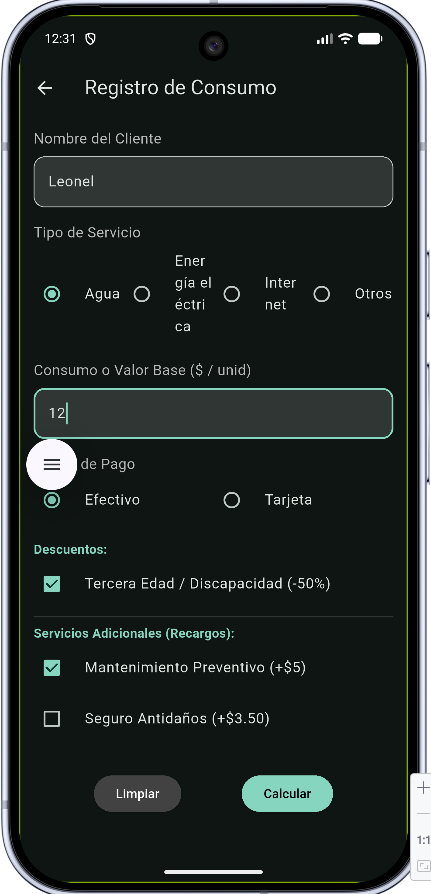
\includegraphics[width=0.4\textwidth]{ejercicio1_ejecucion.png}
\end{center}

\newpage
\subsection{Ejercicio 2: Aplicación 2 - Factura de pago a choferes (pry\_deber2\_act2)}
\textbf{Descripción:}\\
Crear una aplicación móvil para calcular la nómina semanal de una compañía de transporte que cuenta con cinco choferes.

\textbf{Datos requeridos:}\\
De cada chofer se debe registrar:
\begin{itemize}
    \item Nombre.
    \item Horas trabajadas por día durante seis días.
    \item Sueldo por hora.
\end{itemize}

\textbf{Reglas de negocio:}\\
La aplicación debe calcular:
\begin{itemize}
    \item Total de horas trabajadas a la semana por cada chofer.
    \item Sueldo semanal de cada chofer.
    \item Total general que pagará la empresa.
    \item Nombre del chofer que trabajó más horas el día lunes.
    \item Reporte general con todos los datos calculados.
\end{itemize}

\subsubsection{Pseudocódigo}
\begin{verbatim}
Inicio
  Leer N // Número de choferes
  totalEmpresa = 0
  maxHorasLunes = -1
  choferDestacado = ""
  
  Para i desde 1 hasta N Hacer
    Leer nombre, sueldoPorHora, recibeBono, horasDiarias[1..6]
    
    totalHorasChofer = 0
    Para j desde 1 hasta 6 Hacer
      totalHorasChofer = totalHorasChofer + horasDiarias[j]
    FinPara
    
    sueldoSemanal = totalHorasChofer * sueldoPorHora
    Si recibeBono == Verdadero Entonces
      sueldoSemanal = sueldoSemanal + 50.0
    FinSi
    
    totalEmpresa = totalEmpresa + sueldoSemanal
    
    Si horasDiarias[1] > maxHorasLunes Entonces
      maxHorasLunes = horasDiarias[1]
      choferDestacado = nombre
    FinSi
    
    Imprimir "Chofer:", nombre, "Sueldo:", sueldoSemanal
  FinPara
  
  Imprimir "Total a pagar empresa:", totalEmpresa
  Imprimir "Chofer destacado Lunes:", choferDestacado
Fin
\end{verbatim}
\vspace{0.3cm}
Este pseudocódigo describe una lógica de procesamiento mucho más interactiva y de acumulación, donde intervienen arreglos para representar las horas diarias de una jornada semanal de 6 días, además de bucles iterativos que procesan conductor por conductor. Simultáneamente a los cálculos de nómina, se actualiza un registro comparativo para determinar en tiempo real el conductor más activo del primer día (Lunes).

\subsubsection{Diagrama Nassi-Shneiderman}
\vspace{0.5cm}
\begin{center}
\begin{struktogramm}(140, 95)
  \assign{Leer lista de \texttt{choferes}}
  \assign{\texttt{totalEmpresa} $\gets$ 0}
  \assign{\texttt{maxHorasLunes} $\gets$ -1, \texttt{choferDestacado} $\gets$ ""}
  \while{Para cada \texttt{chofer} en \texttt{choferes}}
    \assign{\texttt{totalHoras} $\gets$ suma de \texttt{chofer.horasDiarias}}
    \assign{\texttt{sueldoSemanal} $\gets$ \texttt{totalHoras} * \texttt{chofer.sueldoPorHora}}
    \ifthenelse[15]{1}{1}{\texttt{chofer.recibeBono} == Verdadero}{\textbf{Sí}}{\textbf{No}}
        \assign{\texttt{sueldoSemanal} $\gets$ \texttt{sueldoSemanal} + 50.0}
    \change
    \ifend
    \assign{\texttt{totalEmpresa} $\gets$ \texttt{totalEmpresa} + \texttt{sueldoSemanal}}
    \ifthenelse[15]{1}{1}{\texttt{chofer.horasDiarias}[0] $>$ \texttt{maxHorasLunes}}{\textbf{Sí}}{\textbf{No}}
        \assign{\texttt{maxHorasLunes} $\gets$ \texttt{chofer.horasDiarias}[0]}
        \assign{\texttt{choferDestacado} $\gets$ \texttt{chofer.nombre}}
    \change
    \ifend
  \whileend
  \assign{Imprimir \texttt{totalEmpresa}, \texttt{choferDestacado}}
\end{struktogramm}
\end{center}

\vspace*{1.5cm}
\noindent
El diagrama ilustra el recorrido de la estructura de datos que almacena a los choferes registrados. El bloque cíclico principal encapsula tanto la determinación del sueldo base y la suma del bono especial para cada empleado de forma individual, como también el algoritmo de búsqueda de un máximo, crucial para reportar la eficiencia productiva de la plantilla laboral.

\subsubsection{Código (Lógica Central del Modelo)}
\begin{maccode}{lib/model/chofer\_model.dart}
class Chofer {
  // Atributos: nombre, horasDiarias, sueldoPorHora, etc.
  
  double calcularTotalHoras() => horasDiarias.fold(0, (a, b) => a + b);

  double calcularSueldoSemanal() {
    double base = calcularTotalHoras() * sueldoPorHora;
    return recibeBono ? base + 50.0 : base;
  }
}

class NominaModel {
  final List<Chofer> choferes;
  NominaModel({required this.choferes});

  double calcularTotalEmpresa() {
    return choferes.fold(0, (total, chofer) => 
               total + chofer.calcularSueldoSemanal());
  }

  String obtenerChoferMasHorasLunes() {
    if (choferes.isEmpty) return "No se registraron choferes";
    Chofer destacado = choferes.first;
    for (var chofer in choferes) {
      if (chofer.horasDiarias[0] > destacado.horasDiarias[0]) {
        destacado = chofer;
      }
    }
    return destacado.nombre;
  }
}
\end{maccode}
\vspace{0.3cm}
En la implementación final de Dart, podemos resaltar el uso de las funciones de orden superior y métodos declarativos para iterables (como el método \texttt{fold} aplicado sobre la lista \texttt{horasDiarias} o sobre los propios \texttt{choferes}), lo que nos permite contraer múltiples ciclos for convencionales en elegantes líneas compactas. Asimismo, la clase padre \texttt{NominaModel} orquesta el cálculo general administrando internamente múltiples instancias de un submodelo base llamado \texttt{Chofer}.

\subsubsection{Ejecución}
La siguiente captura evidencia el diseño moderno e iterativo construido en la interfaz gráfica, en donde las tarjetas dinámicas que representan a cada conductor son un claro ejemplo del uso de "moléculas" atómicas inyectadas directamente dentro de una "plantilla" o "página" mayor, logrando una lista de componentes fluidos y reutilizables.
\begin{center}
    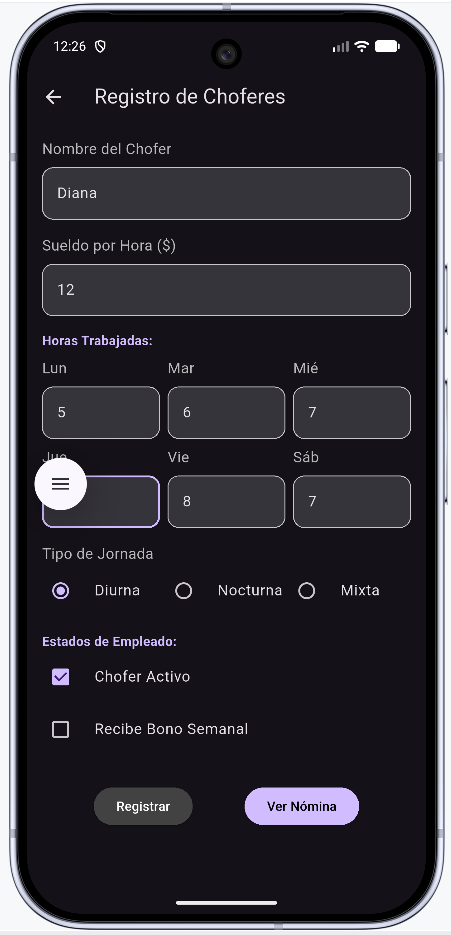
\includegraphics[width=0.4\textwidth]{ejercicio2_ejecucion.png}
\end{center}

\newpage
\section{Conclusiones}
\begin{itemize}
    \item La abstracción de algoritmos mediante pseudocódigos y diagramas Nassi-Shneiderman ha permitido diseñar lógicas estructuradas mucho antes de escribir el código fuente, lo que previene errores semánticos y refactorizaciones durante el desarrollo.
    \item La adopción del patrón MVC en el entorno de desarrollo Flutter ha demostrado ser altamente eficiente para separar la lógica de negocio de la interfaz de usuario. Además, el diseño visual se construyó de manera mucho más modular, aplicando los principios del Diseño Atómico (Atomic Design), separando los \textit{widgets} en átomos, moléculas y organismos, lo que permite una mayor reutilización de código y escalabilidad en los proyectos.
    \item En la resolución de problemas (como el cálculo de facturas y la gestión de nóminas), encapsular la lógica pura dentro del \textit{Modelo} permitió simplificar el código, haciendo que los controladores manejen validaciones de vista y deleguen el comportamiento matemático sin interrupciones.
\end{itemize}

\section{Referencias}
\begin{itemize}
    \item Chapin, N. (1974). \textit{New Format for Flowcharts}. Software: Practice and Experience, 4(4), 341-357.
  \item Google (2024). \textit{Flutter Documentation}. Recuperado de \url{https://docs.flutter.dev/}
  \item Google (2024). \textit{Dart Language Overview}. Recuperado de \url{https://dart.dev/overview}
  \item Google (2024). \textit{Android Studio User Guide}. Recuperado de \url{https://developer.android.com/studio/intro}
    \item Gamma, E., Helm, R., Johnson, R., y Vlissides, J. (1994). \textit{Design Patterns: Elements of Reusable Object-Oriented Software}. Addison-Wesley.
  \item Oracle (2024). \textit{Java Platform, Standard Edition: Java Language Specification}. Recuperado de \url{https://docs.oracle.com/javase/specs/}
\end{itemize}

\section{Anexos}
\subsection{Repositorio de código fuente}

\subsubsection{Enlace principal}
\begin{itemize}
  \item \url{https://github.com/LeonelTQL/moviles/tree/main/pry_deber2}
  \item \url{https://github.com/LeonelTQL/moviles/tree/main/pry_deber2_act2}
\end{itemize}

\end{document}
